\documentclass[12pt,reqno,oneside,pdftex]{formato-puc/puctesis} % For pdflatex
\usepackage{graphicx}
\usepackage{amsmath}
\usepackage{amsfonts}
\usepackage{amssymb}
\usepackage[spanish]{algorithm2e}
\usepackage{fancybox}
\usepackage{float}
\usepackage{times}

\usepackage{color}
\usepackage{fancyvrb}
\newcommand{\VerbBar}{|}
\newcommand{\VERB}{\Verb[commandchars=\\\{\}]}
\DefineVerbatimEnvironment{Highlighting}{Verbatim}{commandchars=\\\{\}}
\usepackage{framed}
\definecolor{shadecolor}{RGB}{248,248,248}
\newenvironment{Shaded}{\begin{snugshade}}{\end{snugshade}}
\newcommand{\AlertTok}[1]{\textcolor[rgb]{0.94,0.16,0.16}{#1}}
\newcommand{\AnnotationTok}[1]{\textcolor[rgb]{0.56,0.35,0.01}{\textbf{\textit{#1}}}}
\newcommand{\AttributeTok}[1]{\textcolor[rgb]{0.77,0.63,0.00}{#1}}
\newcommand{\BaseNTok}[1]{\textcolor[rgb]{0.00,0.00,0.81}{#1}}
\newcommand{\BuiltInTok}[1]{#1}
\newcommand{\CharTok}[1]{\textcolor[rgb]{0.31,0.60,0.02}{#1}}
\newcommand{\CommentTok}[1]{\textcolor[rgb]{0.56,0.35,0.01}{\textit{#1}}}
\newcommand{\CommentVarTok}[1]{\textcolor[rgb]{0.56,0.35,0.01}{\textbf{\textit{#1}}}}
\newcommand{\ConstantTok}[1]{\textcolor[rgb]{0.00,0.00,0.00}{#1}}
\newcommand{\ControlFlowTok}[1]{\textcolor[rgb]{0.13,0.29,0.53}{\textbf{#1}}}
\newcommand{\DataTypeTok}[1]{\textcolor[rgb]{0.13,0.29,0.53}{#1}}
\newcommand{\DecValTok}[1]{\textcolor[rgb]{0.00,0.00,0.81}{#1}}
\newcommand{\DocumentationTok}[1]{\textcolor[rgb]{0.56,0.35,0.01}{\textbf{\textit{#1}}}}
\newcommand{\ErrorTok}[1]{\textcolor[rgb]{0.64,0.00,0.00}{\textbf{#1}}}
\newcommand{\ExtensionTok}[1]{#1}
\newcommand{\FloatTok}[1]{\textcolor[rgb]{0.00,0.00,0.81}{#1}}
\newcommand{\FunctionTok}[1]{\textcolor[rgb]{0.00,0.00,0.00}{#1}}
\newcommand{\ImportTok}[1]{#1}
\newcommand{\InformationTok}[1]{\textcolor[rgb]{0.56,0.35,0.01}{\textbf{\textit{#1}}}}
\newcommand{\KeywordTok}[1]{\textcolor[rgb]{0.13,0.29,0.53}{\textbf{#1}}}
\newcommand{\NormalTok}[1]{#1}
\newcommand{\OperatorTok}[1]{\textcolor[rgb]{0.81,0.36,0.00}{\textbf{#1}}}
\newcommand{\OtherTok}[1]{\textcolor[rgb]{0.56,0.35,0.01}{#1}}
\newcommand{\PreprocessorTok}[1]{\textcolor[rgb]{0.56,0.35,0.01}{\textit{#1}}}
\newcommand{\RegionMarkerTok}[1]{#1}
\newcommand{\SpecialCharTok}[1]{\textcolor[rgb]{0.00,0.00,0.00}{#1}}
\newcommand{\SpecialStringTok}[1]{\textcolor[rgb]{0.31,0.60,0.02}{#1}}
\newcommand{\StringTok}[1]{\textcolor[rgb]{0.31,0.60,0.02}{#1}}
\newcommand{\VariableTok}[1]{\textcolor[rgb]{0.00,0.00,0.00}{#1}}
\newcommand{\VerbatimStringTok}[1]{\textcolor[rgb]{0.31,0.60,0.02}{#1}}
\newcommand{\WarningTok}[1]{\textcolor[rgb]{0.56,0.35,0.01}{\textbf{\textit{#1}}}}

\usepackage[spanish]{babel}
\usepackage[utf8]{inputenc}
%\usepackage[latin1]{inputenc}
                                
\addto\captionsspanish{
  \renewcommand{\contentsname}{INDICE GENERAL}
}
\addto\captionsspanish{
 \renewcommand{\listfigurename}{INDICE DE FIGURAS}
}
\addto\captionsspanish{
 \renewcommand{\listtablename}{INDICE DE TABLAS}
}
\addto\captionsspanish{
 \renewcommand{\chaptername}{CAPITULO}
}
\addto\captionsspanish{
 \renewcommand{\figurename}{Figura}
}
\addto\captionsspanish{
 \renewcommand{\tablename}{Tabla}
}

\newtheorem{definicion}{\bf Definici\'on}[chapter]
\newtheorem{propiedad}{Propiedad}[chapter]
\newtheorem{afirmacion}{Afirmaci\'on}[chapter]
\newtheorem{lema}{\bf Lema}[chapter]
\newtheorem{proposicion}{Proposici\'on}[chapter]
\newtheorem{teorema}{\noindent \bf Teorema}[chapter]
\newtheorem{corolario}{\bf Corolario}[chapter]
\newtheorem{pf}{Demostraci\'on}[chapter]
\newtheorem{ejemplo}{\bf Ejemplo}[chapter]
\newtheorem{comentario}{Comentario}[chapter]

\newcommand\opgrad{\operatorname{grad}}    

% para texlive 2020
\newlength{\cslhangindent}
\setlength{\cslhangindent}{1.5em}
\newenvironment{CSLReferences}
  {}
  {\par}

\begin{document}

\title{Fórmula de la media y la serie geométrica, tesis de ejemplo}
\author{PACHÁ}

\degree       {Magíster en Estadística} 
\advisor      {Nombre del profesor guía}
\committeememberA      {Nombre del miembro del comité 1}
\committeememberB      {Nombre del miembro del comité 2}
\committeememberC      {Nombre del miembro del comité 3}
\date         {Diciembre 2019}
\copyrightname{SIMPLEMENTE PACHÁ}
\copyrightyear{MMXIX}
\dedication   {A mi familia, amigos y personas valiosas de la
universidad}

\PageNumbersFootCentered
\pagenumbering{roman}
\maketitle

\chapter*{AGRADECIMIENTOS}
Esta plantilla de R Markdown se base en la plantilla Latex hecha por
Miguel Torres Torriti. Los agradecimientos se editan directamente en formato-puc/base.tex.
\par

\cleardoublepage
\tableofcontents
\listoffigures          
\listoftables           
\cleardoublepage

\chapter*{RESUMEN}
Un resumen breve

\cleardoublepage % In double-sided printing style makes the next page 
                 % a right-hand page, (i.e. a truly odd-numbered page 
                 % with respect to absolut counting), producing a blank
                 % page if necessary. Added by MTT 20.AUG.2002 

\NoChapterPageNumber           % elimina encabezado - pie de pagina de la
                               % primera pagina de cada capitulo
\pagenumbering{arabic}

\mainmatter

\chapter{NOMBRE DEL CAPITULO 1}

\hypertarget{seccion-1}{%
\section{SECCION 1}\label{seccion-1}}

Texto de ejemplo: Sed ut perspiciatis unde omnis iste natus error sit
voluptatem accusantium doloremque laudantium, totam rem aperiam, eaque
ipsa quae ab illo inventore veritatis et quasi architecto beatae vitae
dicta sunt explicabo. Nemo enim ipsam voluptatem quia voluptas sit
aspernatur aut odit aut fugit, sed quia consequuntur magni dolores eos
qui ratione voluptatem sequi nesciunt. Neque porro quisquam est, qui
dolorem ipsum quia dolor sit amet, consectetur, adipisci velit, sed quia
non numquam eius modi tempora incidunt ut labore et dolore magnam
aliquam quaerat voluptatem. Ut enim ad minima veniam, quis nostrum
exercitationem ullam corporis suscipit laboriosam, nisi ut aliquid ex ea
commodi consequatur? Quis autem vel eum iure reprehenderit qui in ea
voluptate velit esse quam nihil molestiae consequatur, vel illum qui
dolorem eum fugiat quo voluptas nulla pariatur?

\hypertarget{sub-seccion-1}{%
\subsection{SUB-SECCION 1}\label{sub-seccion-1}}

Texto de ejemplo: At vero eos et accusamus et iusto odio dignissimos
ducimus qui blanditiis praesentium voluptatum deleniti atque corrupti
quos dolores et quas molestias excepturi sint occaecati cupiditate non
provident, similique sunt in culpa qui officia deserunt mollitia animi,
id est laborum et dolorum fuga. Et harum quidem rerum facilis est et
expedita distinctio. Nam libero tempore, cum soluta nobis est eligendi
optio cumque nihil impedit quo minus id quod maxime placeat facere
possimus, omnis voluptas assumenda est, omnis dolor repellendus.
Temporibus autem quibusdam et aut officiis debitis aut rerum
necessitatibus saepe eveniet ut et voluptates repudiandae sint et
molestiae non recusandae. Itaque earum rerum hic tenetur a sapiente
delectus, ut aut reiciendis voluptatibus maiores alias consequatur aut
perferendis doloribus asperiores repellat.

\hypertarget{seccion-2}{%
\section{SECCION 2}\label{seccion-2}}

Por completitud incluyo una cita en Bibtex: Bock, Velleman, and De Veaux
(2010) contiene la ecuación de la media ponderada.

También podríamos decir ``la definición de media ponderada es \ldots{}
(Bock, Velleman, and De Veaux 2010).''

\chapter{NOMBRE DEL CAPITULO 2}

\hypertarget{algunas-ecuaciones}{%
\section{ALGUNAS ECUACIONES}\label{algunas-ecuaciones}}

\hypertarget{serie-geomuxe9trica}{%
\subsection{Serie geométrica}\label{serie-geomuxe9trica}}

Sea \(r\in (0,1)\) se tiene que la suma de exponentes consecutivos de
\(r^i\) converge, es decir \begin{equation}
\sum_{i=0}^{\infty} r^i = \frac{1}{1-r}
\end{equation} notamos que \(r\) puede crecer de manera tal que \[
\lim_{r\to \infty} \frac{1}{1-r} = 0
\] o escrito de otra manera \[
\sum_{i=0}^{\infty} r^i = \frac{1}{1-r} \stackrel{r\to \infty}{\longrightarrow} 0
\]

\hypertarget{distribuciuxf3n-normal}{%
\subsection{Distribución Normal}\label{distribuciuxf3n-normal}}

\begin{equation}
\mathcal{N}(\mu,\sigma^2) = \int\limits_{-\infty}^{x} \frac1{\sigma\sqrt{2\pi}}\: \exp{-\frac{1}{2}\left(\frac{t-\mu}{\sigma}\right)^2}\: dt
\end{equation}

\appendix

\chapter{INSERTANDO IMAGENES, TABLAS, CODIGO, ETC}

El código R (se ejecuta sin necesidad de hacer copy paste del resultado
a un archivo tex):

\begin{Shaded}
\begin{Highlighting}[]
\FunctionTok{summary}\NormalTok{(cars)}
\end{Highlighting}
\end{Shaded}

\begin{verbatim}
##      speed           dist       
##  Min.   : 4.0   Min.   :  2.00  
##  1st Qu.:12.0   1st Qu.: 26.00  
##  Median :15.0   Median : 36.00  
##  Mean   :15.4   Mean   : 42.98  
##  3rd Qu.:19.0   3rd Qu.: 56.00  
##  Max.   :25.0   Max.   :120.00
\end{verbatim}

\begin{Shaded}
\begin{Highlighting}[]
\FunctionTok{plot}\NormalTok{(pressure)}
\end{Highlighting}
\end{Shaded}

\begin{figure}
\centering
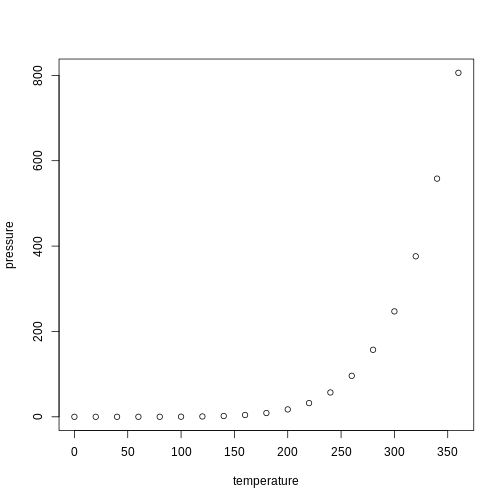
\includegraphics{tesis-rmarkdown_files/figure-latex/pressure-1.pdf}
\caption{Gráfico de presión}
\end{figure}

Tabla con comandos \LaTeX:

\begin{table}[h]
\centering
\begin{tabular}{l*{6}{c}r}
Variable              & Obs 1 & Obs 2 & Obs 3 & Obs 4 & Obs 5\\
\hline
V1 & 6 & 4 & 0 & 2 & 10 \\
V2            & 6 & 3 & 0 & 3 &  8 \\
V3           & 6 & 2 & 1 & 3 &  7 \\
V4     & 6 & 2 & 1 & 3 &  5 \\
\end{tabular}
    \caption{Tabla de ejemplo.}
\end{table}

\chapter*{BIBLIOGRAFIA}

\hypertarget{refs}{}
\begin{CSLReferences}{1}{0}
\leavevmode\hypertarget{ref-bock2010stats}{}%
Bock, David E, Paul F Velleman, and Richard D De Veaux. 2010.
\emph{Stats: Modeling the World}. Addison-Wesley.

\end{CSLReferences}

\end{document}
